% \documentclass[10pt,handout,usenames,dvipsnames,pdf]{beamer}
\documentclass[10pt,usenames,dvipsnames,pdf]{beamer}

\usepackage[portuguese,english]{babel}
\usepackage[backend=biber,style=authoryear-icomp,natbib=true,url=false,doi=true]{biblatex}

\usepackage[notesposition=right,duration=20,lastminutes=5]{pdfpc}

\usepackage[scale=2]{ccicons}

\usepackage{hyperref}
\usepackage{bookmark}

\usepackage{booktabs}
\usepackage{multirow}
\usepackage{graphicx}
\usepackage{csquotes}
\usepackage{float}

\usepackage{tikz}
\usepackage{pgfplots}
\usepackage{pgfplotstable}

\usepackage[ruled,lined]{algorithm2e}

\usepackage{listings}
\usepackage{siunitx}

% Color Definitions (Colourblind friendly)
\definecolor{cb_blue}{RGB}{0, 92, 169}
\definecolor{cb_orange}{RGB}{213, 94, 0}
\definecolor{cb_green}{RGB}{0, 158, 115}
\definecolor{cb_purple}{RGB}{102, 51, 153}
\definecolor{cb_pink}{RGB}{204, 121, 167}
\definecolor{cb_gray}{RGB}{153, 153, 153}
\definecolor{cb_dark_yellow}{RGB}{230, 159, 0}
\definecolor{cb_light_blue}{RGB}{86, 180, 233}
\definecolor{cb_light_yellow}{RGB}{240, 228, 66}
\definecolor{cb_dark_blue}{RGB}{0, 114, 178}

% Code Listings Style
\lstset{ %
  showstringspaces=false,
  language=Python,
  basicstyle=\footnotesize\ttfamily,
  columns=fullflexible,
  keepspaces=true,
  literate={->}{$\rightarrow$}2,
  keywordstyle=\color{cb_blue}\bfseries,
  stringstyle=\color{cb_pink},
  morekeywords={sort, assert, append},
  keywords=[2]{Problem, Solution, Component, LocalMove, 
               Iterable, Hashable, None, int, T, bool, Optional, Timer,
               True, False},
  keywordstyle=[2]\color{cb_green}\bfseries,
  emph={empty_solution, random_solution, id, objective, upper_bound,
        feasible, add_moves, remove_moves, components,
        heuristic_add_move, heuristic_add_moves, random_add_move,
        random_remove_move, add, remove, upper_bound_increment_add,
        upper_bound_increment_remove,objective_increment_add,
        objective_increment_remove, local_moves,random_local_moves_wor,
        random_local_move, step, objective_increment_local, perturb, copy,
        heuristic_value},
  emphstyle=\color{cb_orange},
  xleftmargin=10mm,
}

% Bibliography
\addbibresource{../references.bib}

% PDF Presenter Console (pdfpc) Notes
\setbeamertemplate{note page}{\pagecolor{black!2}\normalsize\insertnote}

% \setbeameroption{hide notes}
\setbeameroption{show notes on second screen=right}

\newcommand<>{\talknote}[1]{\only#2{\note[item]{\textbf{#1}}\relax}}

% PDF Metadata
\hypersetup{
 pdftitle = {Principled Modeling of the Google Hash Code Problems for Meta-Heuristics},
 pdfauthor = {Pedro Miguel Duque Rodrigues},
 pdfsubject = {Master Thesis - Presentation},
 pdfkeywords = {Intelligent Systems, Modeling, Meta-Heuristics},
 pdfproducer = {Latex Beamer with hyperref},
 pdfcreator = {lualatex},
}

% Beamer Theme
\usetheme[progressbar=frametitle,background=light]{metropolis}
\metroset{block=fill}

% Algorithm Style
\SetKwInOut{KwIn}{Input}
\SetKwInOut{KwOut}{Output}
\SetKwComment{Comment}{$\vartriangleright$\ }{}
\DontPrintSemicolon

% Custom Operators
\DeclareMathOperator*{\argmax}{argmax}
\DeclareMathOperator*{\argmin}{argmin}

% Title Page Settings
\title{Principled Modeling of the Google Hash Code Problems for Meta-Heuristics}
\author{Pedro Rodrigues \vspace{0.1cm} \\ \scriptsize Alexandre D. Jesus \\ \and Carlos M. Fonseca \\} 
\date{\footnotesize September 2023}
\institute{University of Coimbra \\ Department of Informatics Engineering}

\begin{document}

\begin{frame}[noframenumbering, plain]
  \titlepage
  \talknote{Welcome the audience}
\end{frame}

\begin{frame}{Outline}
  \tableofcontents
\end{frame}

\section{Introduction}
\begin{frame}{Motivation}
  Combinatorial Optimization problems that often emerge in real-world scenarios:
  \begin{itemize}
    \item Are~\textbf{large} and~\textbf{complex}.
    \item \textbf{Cannot be solved} by~\alert{exact} methods in a~\textbf{reasonable amount of time}.
  \end{itemize}

  The~\alert{Google Hash Code} programming competition invited people
  to solve challenging problems.

  \begin{itemize}
    \item \textbf{Complex problems} inspired by engineering challenges.
    \item Inspired by~\textbf{real-world} scenarios.
    \item \textbf{Well formulated} and can be solved to some extent in a short amount of time.
  \end{itemize}
\end{frame}

\begin{frame}{Motivation}
  \alert{Meta-Heuristics} are methods that~\textquote{guide and intelligently combine subordinate
    heuristics for exploring and exploiting solutions in the search
    space}~(\cite{osman1996metaheuristics}).

  These methods have interesting properties:
  \begin{itemize}
    \item Can often~\textbf{find~\textquote{good} solutions} for hard problems~\textbf{quickly}.
    \item \textbf{General-purpose}, i.e. they can be applied to many problems.
  \end{itemize}

  There is a community interest in studying them and making them more accessible in practice.
\end{frame}

\begin{frame}{Motivation}
  \alert{Modeling} is the process of creating a simplified representation
  or approximation of a real-world system, process, or phenomenon.

  If this process is done in a principled way, it can be standardized in order to provide:
  \begin{itemize}
    \item A~\textbf{structured approach} to problem-solving.
    \item A clear~\textbf{separation} between~\textbf{problems} and~\textbf{solvers}.
  \end{itemize}

  \begin{figure}[h]
    \centering
    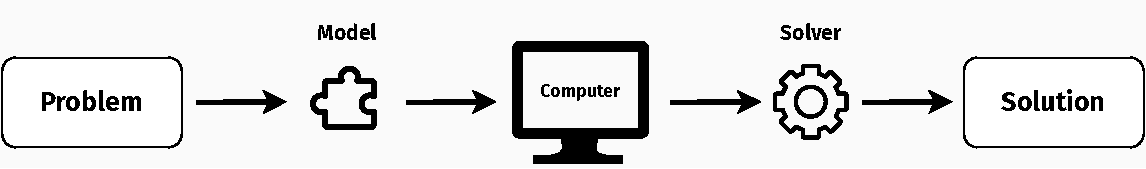
\includegraphics[width=\textwidth,keepaspectratio]{../assets/modelling/modelling-slides.pdf}
    \caption{Principled Modeling Framework}
  \end{figure}
\end{frame}

\begin{frame}{Goals \& Scope}
  The main research questions we outline for this work are:
  \begin{enumerate}
    \item Can existing ideas on modeling frameworks~(\cite{vieira2009uma,fonseca2021nasf4nio,outeiro2021application})
          be formalized into a more practical and complete implementation?

    \item Can general-purpose meta-heuristic solvers be developed
          through the principled modeling framework implementation?

    \item Can Google Hash Code problems be solved effectively using
          this modeling approach?
  \end{enumerate}
\end{frame}

\begin{frame}{Contributions}
  The main contributions of this work are related to the aforementioned research questions, as follows:
  \begin{enumerate}
    \item A practical Python implementation of the principled modeling framework was
          created.

    \item Several meta-heuristic solvers and utilities were developed on top of
          the principled modeling framework implementation.

    \item Several models were developed for two of the Google Hash Code problems.
  \end{enumerate}
\end{frame}

% TODO: Other Contributions

\section{Background}
\begin{frame}{Optimization}

  \begin{block}{Optimization Problem}
    An optimization problem is a tuple $(\mathcal{S}, f)$, where
    $\mathcal{S}$ is a set containing all feasible solutions, and $f$ is an
    objective (cost) function, with a mapping such that:
    \begin{equation*}
      f \colon \mathcal{S} \longrightarrow \mathbb{R}
    \end{equation*}
  \end{block}

  \begin{block}{Combinatorial Optimization Problem}
    A combinatorial optimization problem is an optimization problem where the
    set $\mathcal{S}$ of feasible solutions is finite.
  \end{block}

  In this work we assume without loss of generality a maximizing objective function.
\end{frame}

\begin{frame}{Ground Set}

  \begin{block}{Ground Set}
    The ground set of a CO problem is a finite set of
    components $\mathcal{G} = \{c_1, c_2, \ldots, c_k\}$, such that every solution to the
    problem, feasible or not, can be defined as a subset of $\mathcal{G}$.
  \end{block}

  \begin{block}{Empty Solution}
    A solution $s \in 2^\mathcal{G}$, where $2^\mathcal{G}$ denotes the powerset of $\mathcal{G}$,
    is said to be an empty solution if $s = \emptyset$.
  \end{block}

  \begin{block}{Partial Solution}
    A solution $s \in 2^\mathcal{G}$ is said to be a
    partial solution if there is a feasible solution $s' \in \mathcal{S}$ such
    that $s' \supseteq s$.
  \end{block}

  \begin{block}{Complete Solution}
    A feasible solution $s \in \mathcal{S}$ is said
    to be a complete solution if there is no feasible solution $s' \in
      \mathcal{S}$ such that $s' \supset s$.
  \end{block}
\end{frame}

\begin{frame}{Bounds}
  The usage of~\alert{bounds}, particularly the~\emph{upper bound} in a maximization setting,
  is beneficial as it aids in:

  \begin{itemize}
    \item The evaluation of infeasible solutions.
    \item The measurement of a candidate solution's potential.
  \end{itemize}

  \begin{block}{Upper Bound}
    An upper bound of a (partial) solution $s \in 2^\mathcal{G}$ is any numeric
    value given by a function $\Phi_\text{ub}\colon 2^{\mathcal{G}} \rightarrow
      \mathbb{R} $ such that:
    \begin{equation*}
      \forall s' \in \mathcal{S} \land s' \supseteq s \colon f(s') \le \Phi_\text{ub}(s)
    \end{equation*}
  \end{block}
\end{frame}

\begin{frame}[fragile]{Constructive Search}
  \alert{Constructive Search} is a procedure for optimization that operates as follows:

  \begin{itemize}
    \item Initiate the process with an empty or partial solution
    \item Add a component from the ground set to the solution.
    \item Repeat the process until no more (feasible) components are available.
  \end{itemize}

  \begin{center}
    \scalebox{0.75}{%  
      \begin{algorithm}[H]
        \KwIn{Ground Set ($\mathcal{G}$)}
\KwOut{Solution ($s$)}

$s$ $\gets$ $\emptyset$\;
$C$ $\gets$ $\{$  $c\in \mathcal{G} \setminus s$ $|$ $s \cup \{c\}$ \texttt{is feasible} $\}$ \;
\While{$C \neq \emptyset$}{
  $c$ $\gets$ \texttt{SelectComponent($C$)}\;
  $s$ $\gets$ $s \cup \{c\}$\;
  $C$ $\gets$ $\{$  $c\in \mathcal{G} \setminus s$ $|$ $s \cup \{c\}$ \texttt{is feasible} $\}$ \;
}
\Return{$s$}

        \caption{Constructive Search Procedure}
      \end{algorithm}
    }
  \end{center}
\end{frame}


\begin{frame}{Local Search}
  \alert{Local Search} is a procedure for optimization that operates as follows:

  \begin{itemize}
    \item Start with a feasible solution to the problem.
    \item Apply local moves and perturbations to the solution, thus exploring candidate solutions in the neighborhood.
    \item Repeat the process until the solution cannot be further improved.
  \end{itemize}

  \begin{center}
    \scalebox{0.75}{%  
      \begin{algorithm}[H]
        % Local Search Procedure (algorithm2e pseudocode)

\KwIn{Solution ($s'$)}
\KwOut{Solution ($s$)}

\SetKwFunction{LocalMoves}{\texttt{LocalMoves}}
\SetKwFunction{SelectLocalMove}{\texttt{SelectLocalMove}}
\SetKwFunction{Step}{\texttt{Step}}
\SetKwFunction{Perturb}{\texttt{Perturb}}

$s$ $\gets$ $s'$\;
$\mathcal{M}$ $\gets$ \LocalMoves{$s$}\;
\While{$\mathcal{M} \neq \emptyset$ }{
  $m$ $\gets$ \SelectLocalMove{$\mathcal{M}$}\;
  $s$ $\gets$ \Step{$s, m$}\;
  $s$ $\gets$ \Perturb{$s$} \Comment*[f]{Optional}\;
  $\mathcal{M}$ $\gets$ \LocalMoves{$s$}
}
\Return{ $s$ }
        \caption{Local Search Procedure}
      \end{algorithm}
    }
  \end{center}
\end{frame}

\begin{frame}{Meta-Heuristics}
  The following~\alert{meta-heuristics}, were analyzed and implemented in the context
  of this work.
  \begin{itemize}
    \item \emph{Beam Search}
    \item \emph{Iterated Greedy}
    \item \emph{Greedy Randomized Adaptive Search Procedure}
    \item \emph{Ant Colony Optimization}
    \item \emph{Hill-Climbing}
    \item \emph{Iterated Local Search}
    \item \emph{Simulated Annealing}
    \item \emph{Tabu Search}
  \end{itemize}

\end{frame}

\section{Principled Modeling Framework}
\begin{frame}{ Frameworks}
  The following frameworks served as~\textbf{references} for our implementation.

  \begin{description}
    \item[POF] Python Optimization Framework~(\cite{vieira2009uma})
    \item[nasf4nio] Not Another Software Framework for Nature-Inspired Optimization~(\cite{fonseca2021nasf4nio})
    \item[nasf4nio-cs] Not Another Software Framework for Nature-Inspired Optimization --- Constructive Search~(\cite{outeiro2021application})
  \end{description}
\end{frame}

\begin{frame}{Modeling}
  In the context of~\alert{modeling} for~\emph{meta-heuristics}, the following aspects are
  considered relevant:
  \begin{itemize}
    \item \emph{Problem Instance}
    \item \emph{Solution}
    \item \emph{Construction Rules}
    \item \emph{Objective Function \& Bounds}
    \item \emph{Combinatorial Structure (Components)}
    \item \emph{Neighborhood Structure (Local Moves)}
  \end{itemize}
\end{frame}

\begin{frame}{Data Structures}
  The following~\textbf{data structures} constitute the foundation of the framework:

  \begin{description}
    \item[Problem] Holds immutable data that fully characterizes the problem instance.

    \item[Solution] Characterizes a solution for the problem and serves as the mutable state that
      the solver can modify during the optimization process.

    \item[Component] Characterizes any component within the ground set of a given problem.

    \item[LocalMove] Characterizes any local move that can be applied to a solution
  \end{description}

  Notably, these are implemented as~\alert{Python classes}.
\end{frame}

\begin{frame}{Specification}
  The following~\textbf{operations} are provided in an interface between the model and the solvers.

  \begin{itemize}
    \item Problem
          \begin{itemize}
            \item Create Empty Solution~(\texttt{empty\_solution})
          \end{itemize}
    \item Solution
          \begin{itemize}
            \item Enumerate Components~(\texttt{add\_moves},~\texttt{heuristic\_add\_move},~...)
            \item Enumerate Local Moves~(\texttt{local\_moves},~...)
            \item Apply Component~(\texttt{add},~\texttt{remove})
            \item Apply Local Move~(\texttt{step})
            \item Perturb Solution~(\texttt{perturb})
            \item Inspect Solution~(\texttt{objective},~\texttt{upper\_bound})
          \end{itemize}
    \item Component
          \begin{itemize}
            \item Get Identifier~(\texttt{id})
          \end{itemize}
  \end{itemize}

  These operations encompass a variety of~\alert{methods} present in each of the aforementioned classes.
\end{frame}

\begin{frame}[fragile]{Solver Development}
  Solvers call upon the operations defined in the specification in order to find solutions.

  \begin{block}{Heuristic Construction Solver Implementation}
    \begin{center}
      \scalebox{0.95}{
        \lstinputlisting{../assets/code/hc.py}
      }
    \end{center}
  \end{block}

\end{frame}

\section{Google Hash Code Competition}
\begin{frame}{Attendance}
  \begin{figure}[ht]
    \begin{tikzpicture}

  % Data
  \pgfplotstableread{
    Label Qualification Final
    2014 100 54
    2015 230 65
    2016 1050 51
    2017 2815 50
    2018 3012 40
    2019 6672 41
    2020 10725 45
    2021 9003 38
    2022 10177 39
  }\data

  % Legend Style
  \pgfplotsset{
    /pgfplots/area legend/.style={
        /pgfplots/legend image code/.code={
            \fill[##1] (0cm,0.6em) rectangle (2*\pgfplotbarwidth,-0.3em);
          },
      },
  }

  \begin{axis}[
      xlabel = {Year},
      ylabel = {Teams},
      ybar,
      ymin=0,
      opacity=0.8,
      xtick=data,area legend,
      ymode=log,
      width=0.8\textwidth,
      height=\axisdefaultheight,
      legend style={cells={anchor=west}, legend pos=north west, font=\scriptsize},
      x tick label style={font=\scriptsize},
      y tick label style={font=\scriptsize},
      xticklabels from table={\data}{Label},
      xticklabel style={text width=2cm,align=center},
    ]
    % Qualification Round
    \addplot [fill=cb_dark_blue] table [y=Qualification, meta=Label, x expr=\coordindex] {\data};
    \addlegendentry{Qualification Round}

    % Final Round
    \addplot [fill=cb_orange] table [y=Final, meta=Label, x expr=\coordindex] {\data};
    \addlegendentry{Final Round}
  \end{axis}
\end{tikzpicture}
    \caption{Google Hash Code Competition Attendance 2014-2022}
    \label{fig:hashcode-attendance}
  \end{figure}
\end{frame}

\begin{frame}{Problems}
  To better understand the~\alert{Google Hash Code} problems a comprehensive
  analysis was conducted to understand the key properties and similarities with
  well-known literature problems.

  \begin{table}[ht]
    \resizebox{0.9\textwidth}{!}{% 
      \begin{tabular}{@{}cccccccc@{}}
        \toprule
        \multirow{2}{*}{\textbf{Problem}} & \multicolumn{7}{c}{\textbf{Categories}}                                                                                    \\
        \cmidrule{2-8}
        {}                                & Assignment                              & Knapsack   & Coverage   & Vehicle Routing & Simulation & Scheduling & Packing    \\ \midrule
        Street View Routing               &                                         &            & \checkmark & \checkmark      &            &            &            \\
        Optimize a Data Center            & \checkmark                              & \checkmark &            &                 &            &            &            \\
        Loon                              &                                         &            & \checkmark & \checkmark      & \checkmark &            &            \\
        Delivery                          &                                         &            &            & \checkmark      &            &            &            \\
        Satellites                        & \checkmark                              &            & \checkmark &                 & \checkmark &            &            \\
        Streaming Videos                  & \checkmark                              & \checkmark &            &                 &            &            &            \\
        Router Placement                  &                                         &            & \checkmark &                 &            &            &            \\
        Self-Driving Rides                & \checkmark                              &            &            & \checkmark      & \checkmark &            &            \\
        City Plan                         &                                         &            &            &                 &            &            & \checkmark \\
        Photo Slideshow                   &                                         &            &            &                 &            & \checkmark &            \\
        Compiling Google                  &                                         &            &            &                 &            & \checkmark &            \\
        Book Scanning                     & \checkmark                              & \checkmark & \checkmark &                 &            & \checkmark &            \\
        Assembling Smartphones            & \checkmark                              &            &            &                 &            & \checkmark &            \\
        Traffic Signaling                 &                                         &            &            &                 & \checkmark &            &            \\
        Software Engineering at Scale     &                                         &            &            &                 &            & \checkmark &            \\
        Mentorship and Teamwork           &                                         &            &            &                 &            & \checkmark &            \\
        Santa Tracker                     &                                         &            &            & \checkmark      &            &            &            \\ \bottomrule
      \end{tabular}
    }
    \caption{Categorization of Google Hash Code Problems}
    \label{tab:hashcode-summary}
  \end{table}
\end{frame}

\section{Optimize a Data Center Problem}
\begin{frame}{Problem}
  This problem entails optimizing the placement of servers in a data center.

  \begin{itemize}
    \item The data center is modeled as a series of rows, each containing several
          slots in which servers can be placed.
    \item Certain slots may be unavailable due to other installations within the data
          center.
    \item Servers must be logically assigned to pools contributing with their (computing) capacity.
  \end{itemize}
\end{frame}

\begin{frame}{Example --- Data Center}
  \begin{figure}[h]
    \centering
    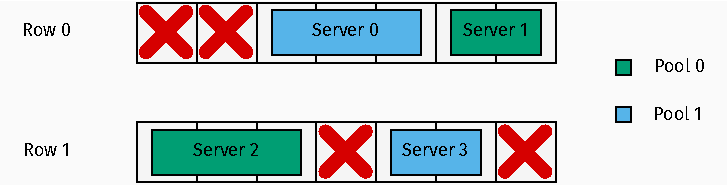
\includegraphics[width=0.9\textwidth,keepaspectratio]{../assets/dc/dc-slides.pdf}
    \caption{Example Data Center Layout}
  \end{figure}

  \begin{table}[ht]
    \centering
    \begin{tabular}{ccc}
      \toprule
      Server & Size & Capacity \\ \midrule
      1      & 3    & 2        \\
      2      & 2    & 5        \\
      3      & 3    & 10       \\
      4      & 2    & 3        \\ \bottomrule
    \end{tabular}
    \caption{Server Properties}
  \end{table}
\end{frame}

\begin{frame}{Guaranteed Capacity}
  The guaranteed capacity is a measure of the remaining computing capacity
  available for a given pool in the event that at most one arbitrary row of the
  data center becomes inoperable.

  \begin{equation*}
    \begin{aligned}
      gc_p(x)     = & \sum_{m=1}^\mathcal{M} \sum_{r=1}^\mathcal{R} \sum_{i \in \mathcal{I}^{r}} c_m \cdot x_{m,p,i} - \max_{r=1}^\mathcal{R} \sum_{m=1}^\mathcal{M} \sum_{i \in \mathcal{I}^r} c_m \cdot x_{m,p,i} \\
    \end{aligned}
  \end{equation*}
  Where,
  \begin{itemize}
    \item $\mathcal{M}$ is the number of servers.
    \item $\mathcal{R}$ is the number of rows.
    \item $\mathcal{I}^{r}$ is a set containing the segment IDs for a given row $r$.
    \item $c_{m}$ is the computing capacity of the server $m$.
    \item $x_{m, p, i}$ is a binary variable indicating whether the server,~$m$, is assigned (1) or not (0) to pool,~$p$, and segment~$i$.
  \end{itemize}
\end{frame}

\begin{frame}{Example --- Guaranteed Capacity}
  \begin{figure}[h]
    \centering
    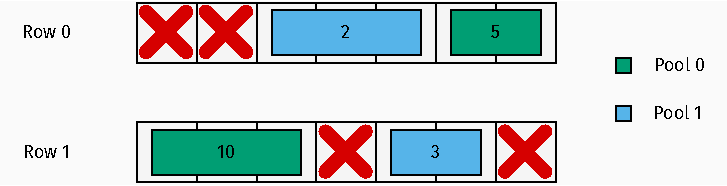
\includegraphics[width=0.9\textwidth,keepaspectratio]{../assets/dc/dc-slides-capacity.pdf}
    \caption{Example Data Center Layout (Capacities Only)}
  \end{figure}

  \begin{table}[ht]
    \centering
    \begin{tabular}{@{\extracolsep{4pt}}cccc}
      \toprule
      Pool & Row 1 & Row 2 & Guaranteed Capacity \\ \midrule
      1    & 5     & 10    & 5                   \\
      2    & 2     & 3     & 2                   \\
      \bottomrule
    \end{tabular}
    \caption{Guaranteed Capacities}
  \end{table}
\end{frame}

\begin{frame}{Problem Formulation}
  \begin{equation*}
    \begin{aligned}
      \max\ f(x)   & = \min_{p=1}^\mathcal{P}{gc_{p}(x)}                                                                                                \\
      \text{s.t. } & \sum_{p=1}^{\mathcal{P}} \sum_{r=1}^{\mathcal{R}} \sum_{i \in \mathcal{I}^{r}} x_{m,p,i} \le 1 & \forall\ m=1,\ldots,\mathcal{M}   \\
                   & \sum_{m=1}^{\mathcal{M}} \sum_{p=1}^{\mathcal{P}} \ell_m \cdot x_{m,p,i} \le \mathcal{L}_{i}   & \forall\  i=1,\ldots, \mathcal{I} \\
                   & x \in {\{0,1\}}^{\mathcal{M} \times \mathcal{P} \times \mathcal{R}}                                                                \\
    \end{aligned}
  \end{equation*}
  Where,
  \begin{itemize}
    \item $\mathcal{P}$ is the number of pools
    \item $\mathcal{I}$ is the number of segments
    \item $\mathcal{L}_{i}$ is the size of segment $i$
    \item $l_{m}$ is the size of the server $m$.
  \end{itemize}
\end{frame}

\begin{frame}{Example --- Objective}
  \begin{figure}[h]
    \centering
    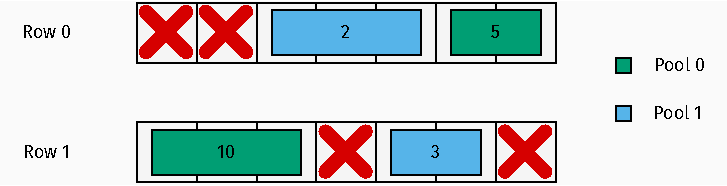
\includegraphics[width=0.9\textwidth,keepaspectratio]{../assets/dc/dc-slides-capacity.pdf}
  \end{figure}

  \begin{table}[ht]
    \centering
    \begin{tabular}{@{\extracolsep{4pt}}ccccc}
      \toprule
      Pool & Row 1 & Row 2 & Guaranteed Capacity & \textbf{$f(x)$}              \\ \midrule
      1    & 5     & 10    & 5                   &                              \\
      2    & 2     & 3     & 2                   & \multirow{-2}{*}{\textbf{2}} \\
      \bottomrule
    \end{tabular}
    \caption{Guaranteed Capacities \& Objective Value}
  \end{table}
\end{frame}

\begin{frame}{Modeling --- Problem, Solution and Component}
  The~\alert{problem} is characterized by the set of available servers, along with
  their respective sizes and capacities, the number of resource pools to be
  created, and the set of segments.

  A~\alert{solution} is characterized by a collection of server assignments to
  pools and segments.

  A~\alert{component} is characterized by a tuple containing a server
  a pool and a segment or just a server (indicating that is forbidden from being assigned).
\end{frame}

\begin{frame}{Modeling --- Construction Rules}
  Three component enumeration strategies were considered:

  \begin{itemize}
    \item \textbf{Standard:} Enumerate all feasible combinations of assignments
          of servers to pools and segments.
    \item \textbf{Sequential:} For one server at a time enumerate all feasible
          assignments to pools and segments.
    \item \textbf{Heuristic:} Select an order for the servers pools and segments
          and enumerate all possible assignments following that order.
  \end{itemize}

  Notably, the component associated with the action of forbidding a server is
  always feasible in any enumeration.
\end{frame}

\begin{frame}{Modeling --- Upper Bound}
  The first upper bound devised for this problem is calculated in through the following steps:
  \begin{enumerate}
    \item \textbf{Relax Segments Constraint:} Remove one row and treat the total available slots in all other rows as a knapsack.

    \item \textbf{Optimize Computing Capacity:} Find the best computing capacity achievable by placing servers in this knapsack.

    \item \textbf{Estimate Guaranteed Capacity:} Divide the capacity by the total number of pools for an optimistic guaranteed capacity estimate.

    \item \textbf{Apply Correction:} If this estimate exceeds the capacity already assigned to any pool.

    \item \textbf{Iterate and Determine Upper Bound:} Repeat these steps for all
          remaining rows, and the upper bound is the minimum value for the guaranteed
          capacity obtained through this process.
  \end{enumerate}

\end{frame}

\begin{frame}{Modeling --- Upper Bound}
  The second upper bound is a slight variation of the previous bound where
  instead of selecting the minimum value in each iteration, a~\textbf{vector containing
    the minimum value for each pool} is kept.

  The~\textbf{upper bound} value is given by this~\textbf{vector sorted in increasing order}.

  Notably, the objective function must be updated where a sorted vector
  containing all the guaranteed capacities serves as the objective value.

  \begin{table}[ht]
    \centering
    \begin{tabular}{@{\extracolsep{4pt}}ccccc}
      \toprule
      Pool & Row 1 & Row 2 & Guaranteed Capacity & \textbf{$f(x)$}                   \\ \midrule
      1    & 5     & 10    & 5                   &                                   \\
      2    & 2     & 3     & 2                   & \multirow{-2}{*}{\textbf{(2, 5)}} \\
      \bottomrule
    \end{tabular}
    \caption{Guaranteed Capacities \& Objective Value}
  \end{table}
\end{frame}

\begin{frame}{Modeling --- Local Moves}
  The~\alert{local moves} considered for this problem are as follows:

  \begin{enumerate}
    \item \textbf{Assigning a server} to a pool and segment if there is an available one.
    \item \textbf{Removing a server} from a segment.
    \item \textbf{Changing the segment} to which a particular server is allocated.
    \item \textbf{Changing the pool} to which a server is allocated, moving it to a different pool.
    \item \textbf{Swapping the pools} of two assigned servers.
    \item \textbf{Swapping the segments} of two assigned servers.
  \end{enumerate}
\end{frame}

\begin{frame}{Results}
  We were able to achieve a objective value of~\alert{386} on the single instance that was
  available through a~\textbf{simple constructive meta-heuristic}.

  Then an~\textbf{Iterated Local Search} meta-heuristic was applied to further
  exploit this solution. The objective value obtained through this process
  was~\alert{410}, which would have placed us in~\textbf{1st place} on the
  competition leaderboard.

  Notably, the best known objective value is~\textbf{408}.
\end{frame}

\section{Book Scanning Problem}
\begin{frame}{Problem}
  This problem entails the setup of scanning pipeline for books.

  \begin{itemize}
    \item There are libraries housing various books. Before any scanning can commence, each
          library needs to register for the scanning process. Once registered, each
          library is allowed to scan a certain number of books daily, until global deadline.
    \item Only one library can undergo the sign-up process at any given time.
    \item Each book, when scanned, contributes a specific score.
  \end{itemize}

\end{frame}

\begin{frame}{Example --- Book Scanning}
  \begin{figure}[h]
    \centering
    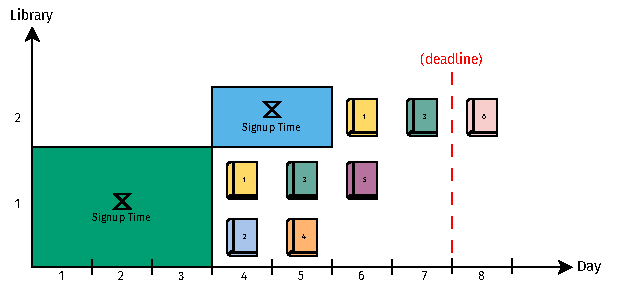
\includegraphics[width=0.8\textwidth,keepaspectratio]{../assets/bs/bs-example-slides.pdf}
    \caption{Book Scanning Example}
  \end{figure}

  \begin{table}[ht]
    \centering
    \begin{tabular}{ccccccc}
      \toprule
      \textbf{Book}  & 1 & 2 & 3 & 4 & 5 & 6 \\ \midrule
      \textbf{Score} & 3 & 1 & 5 & 4 & 7 & 1 \\
      \bottomrule
    \end{tabular}
    \caption{Book Scores}
  \end{table}
\end{frame}

\begin{frame}{Problem Formulation}
  \begin{equation*}
    \begin{aligned}
      \max\ f(x) =\  & \sum_{b = 1}^{\mathcal{B}}{s_{b} \cdot \min\left(\sum_{i = 1}^{\mathcal{I}}{x_{b, \phi_{i}^\mathcal{I}}} , 1\right)}                                                                     \\
      \text{s.t }    & \sum_{b = 1}^{\mathcal{B}}{x_{b, \phi_{i}^\mathcal{I}}} \leq r_{i} \cdot \left(\mathcal{D} - \sum_{k = 1}^{i}{t_{\phi_{k}^\mathcal{I}}} \right) \quad \forall i = 1, \ldots, \mathcal{I} \\
                     & \sum_{i = 1}^{\mathcal{I}}{t_{\phi_{i}^\mathcal{I}}} \leq \mathcal{D}                                                                                                                    \\
    \end{aligned}
  \end{equation*}
  Where,
  \begin{itemize}
    \item $\mathcal{B}$ is the number of books.
    \item $\mathcal{D}$ is the global deadline.
    \item $\mathcal{I}$ and $\phi^\mathcal{I}$ are the number and order of signed-up libraries.
    \item $t_{i}$ and $r_{i}$ are the sign-up time and book scanning rate of library $i$.
    \item $s_{b}$ is the score of book $b$.
    \item $x_{b,i}$ is binary variable indicating if a book, $b$, is assigned (1) or not (0) to library $i$.
  \end{itemize}
\end{frame}


\begin{frame}{Example --- Objective}
  \begin{figure}[h]
    \centering
    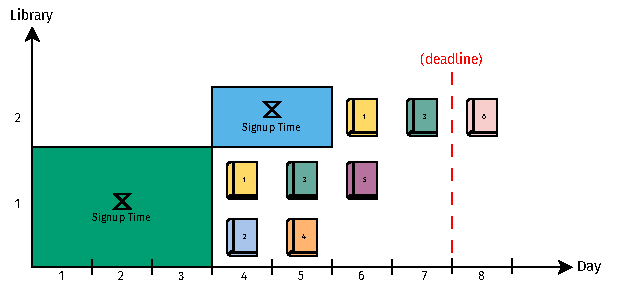
\includegraphics[width=0.8\textwidth,keepaspectratio]{../assets/bs/bs-example-slides.pdf}
  \end{figure}
  \begin{table}
    \begin{tabular}{cc}
      \begin{minipage}{0.5\textwidth}
        \begin{table}[ht]
          \centering
          \begin{tabular}{ccccccc}
            \toprule
            \textbf{Book}  & 1          & 2          & 3          & 4          & 5          & 6 \\ \midrule
            \textbf{Score} & \textbf{3} & \textbf{1} & \textbf{5} & \textbf{4} & \textbf{7} & 1 \\
            \bottomrule
          \end{tabular}
        \end{table}
      \end{minipage}
       &
      \begin{minipage}[b]{0.5\textwidth}
        \centering
        \begin{equation*}
          f(x) = 3 + 1 + 5 + 4 + 7 = 20
        \end{equation*}
      \end{minipage}
    \end{tabular}
    \caption{Book Scores \& Objective Value}
  \end{table}
\end{frame}

\begin{frame}{Modeling --- Problem, Solution and Component}
  The~\alert{problem} is characterized by the set of all libraries available, along with
  their sign-up times, book shipping rate, and list of books that can be shipped,
  the scores for all the books, and the deadline.

  A~\alert{solution} is characterized by a collection of assignments of books
  to libraries and the order in which libraries are scanned.

  A~\alert{component} is characterized by a tuple containing a book and a library or
  a tuple containing two libraries (denoting the sign-up order).
\end{frame}

\begin{frame}{Modeling --- Construction Rules}
  Two component enumeration strategies were considered:
  \begin{itemize}
    \item \textbf{Standard:} Enumerate all the books that can be scanned by all signed-up libraries
          as well as all libraries that can be signed-up until the deadline.
    \item \textbf{Sequential:} Enumerate only the books of the last signed-up library and all the libraries
          that can still be signed-up.
  \end{itemize}
\end{frame}

\begin{frame}{Modeling -- Upper Bound}
  The upper bounds were devised for this problem are as follows:
  \begin{enumerate}
    \item \textbf{Individual Library Knapsacks:} In this approach, we treat the
          number of books each library can scan before the deadline as an individual
          knapsack. The bound value for each library is calculated as the sum of
          scores from the best books that are yet to be scanned. The
          global upper bound is then determined by summing up the bound values for
          each library.

    \item \textbf{Combined Knapsack for All Libraries:} Consider a single
          knapsack representing the total number of books that can be scanned by
          all libraries combined until the deadline.
  \end{enumerate}
\end{frame}

\begin{frame}{Modeling -- Local Moves}
  The~\alert{local moves} considered for this problem are:

  \begin{enumerate}
    \item \textbf{Adding a book} to the set of books to be scanned by a given library.
    \item \textbf{Removing a book} from the set of books that were going to be scanned by a library.
    \item \textbf{Swapping books between libraries}.
    \item \textbf{Removing a book} from the list of books to be scanned by a library and
          \textbf{adding that book to another library}. If possible, ~\textbf{replace the removed book} in
          the first library~\textbf{with another one} that is available there.
  \end{enumerate}
\end{frame}

\begin{frame}{Modeling --- Two-Phase Approach}
  Use a meta-heuristic to choose an order for the libraries and solve the book assignment problem optimally.

  Notably, the assignment problem can be modeled as bipartite graph and solved with any
  \textbf{min cost max-flow} solver.

  \begin{figure}[h]
    \centering
    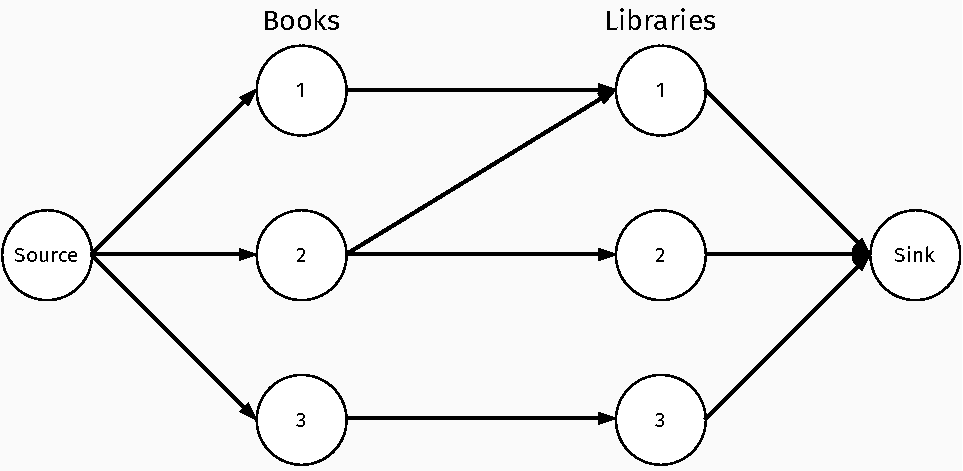
\includegraphics[width=0.8\textwidth,keepaspectratio]{../assets/bs/bs-graph-slides.pdf}
    \caption{Assignment Problem Modeled as a Bipartite Graph}
  \end{figure}
\end{frame}

\begin{frame}{Modeling --- Two-Phase Approach Local Moves}
  After the book assignment the solution can be further improved through
  the following~\alert{local moves}:
  \begin{enumerate}
    \item \textbf{Reverse the sign-up order} between two libraries.
    \item \textbf{Change the positions of two libraries} in the order adjusting the
          sign-up times of every library in between.
    \item \textbf{Select one library to remove and add another library} that is not
          currently considered in that position, if possible.
  \end{enumerate}
\end{frame}

\begin{frame}{Results}
  The best objective values for the five instance of this problem were obtained using the
  \textbf{two-phase} approach, as illustrated in the table below:

  \begin{table}[ht]
    \centering
    \begin{tabular}{@{\extracolsep{4pt}}lcc@{\extracolsep{4pt}}}
      \toprule
      Instance                           & Objective Value & Best Known Objective Value \\ \midrule
      \textquote{Read On}                & \num{5822900}   & \num{5822900}              \\
      \textquote{Incunabula}             & \num{5689822}   & \num{5690888}              \\
      \textquote{Tough Choices}          & \num{5028530}   & \num{5107113}              \\
      \textquote{So many books}          & \num{5208455}   & \num{5237345}              \\
      \textquote{Libraries of the world} & \num{5328034}   & \num{5348248}              \\
      \bottomrule
    \end{tabular}
    \caption{Book Scanning Best Results}
  \end{table}

  Remarkably, this objective value would have placed us in~\textbf{33rd}
  place~(out of 10716 teams) on the competition leaderboard.
\end{frame}

\section{Conclusion \& Future Work}
\begin{frame}{Conclusion}
  In this work we were able to:

  \begin{itemize}
    \item Implement a modeling framework for meta-heuristics.
    \item Implement several meta-heuristic solvers.
    \item Develop models two Google Hash Code problems that achieve competitive results.
  \end{itemize}
\end{frame}

\begin{frame}{Future Work}
  The following topics can be considered as interesting future work directions:
  \begin{itemize}
    \item Development of more Google Hash Code problem models.
    \item Implementation of more Meta-Heuristic solvers.
    \item Experimental evaluation of Meta-Heuristics.
  \end{itemize}

\end{frame}

\begin{frame}[standout]
  \talknote{Thank the audience for being awake.}
  Questions?
\end{frame}

\appendix

\section{References}
\label{sec:references}

\begin{frame}[allowframebreaks]{References}
  \printbibliography[heading=none]
\end{frame}

\end{document}
